\subsection{数据描述与任务DNA来源}
我们从O*NET 30.1文本数据库中提取SOC 15-1252.00的任务陈述和任务评分，并根据重要性（IM）和任务频率（FT）评分计算任务权重。\cite{onet2025database}

\begin{table}[htbp]
\centering
\caption{任务DNA的数据来源与变量}
\label{tab:data_sources_task_dna}
\begin{tabular}{@{}p{3.4cm} p{7.4cm} p{3.2cm}@{}}
\toprule
变量/数据 & 描述 & 来源 \\
\midrule
O*NET任务陈述 & SOC 15-1252.00的任务文本和标识符 & O*NET 30.1数据库\newline \cite{onet2025database} \\
O*NET任务评分（IM, FT） & 用于计算任务权重的重要性和频率评分 & O*NET 30.1数据库\newline \cite{onet2025database} \\
任务DNA CSV & 包含IM、FR、权重和基于规则的s/c的处理后任务表 & 基于O*NET 30.1衍生\newline \cite{onet2025database} \\
\bottomrule
\end{tabular}
\end{table}

\begin{figure}[htbp]
\centering
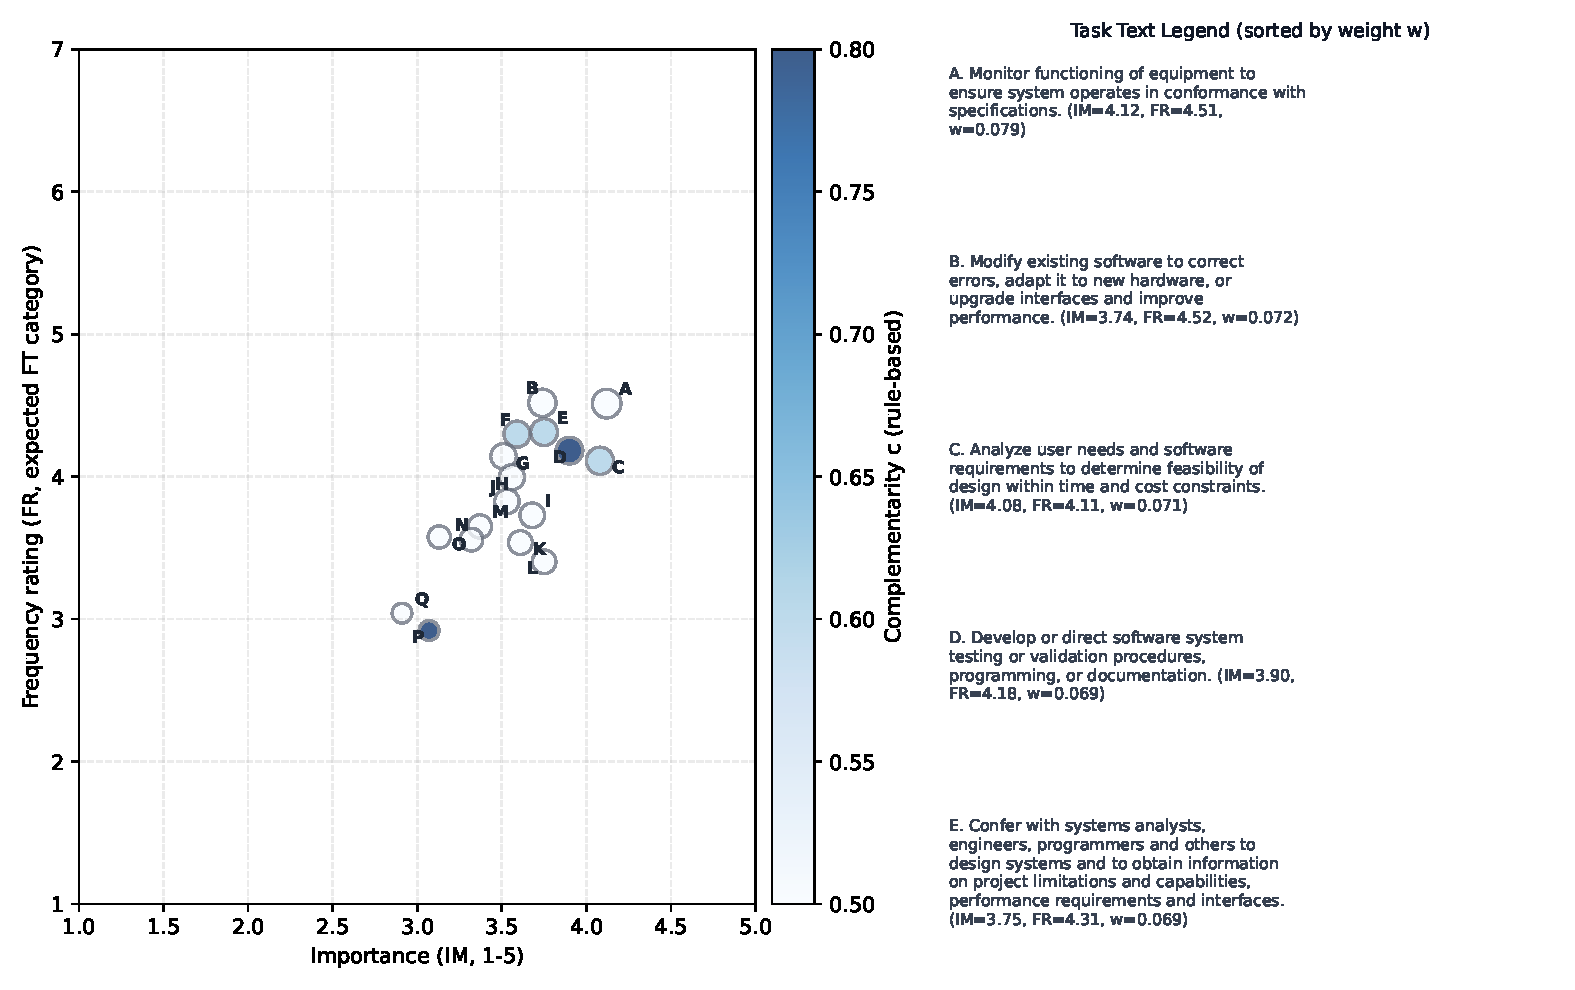
\includegraphics[width=0.82\textwidth]{figures/task_dna_15-1252_weights.pdf}
\caption{软件开发人员（SOC 15-1252.00）的任务级IM--FR暴露度。气泡大小编码归一化任务权重 $w$，颜色编码基于规则的互补性 $c$，边缘粗细反映基于规则的替代性 $s$。字母标签映射到任务文本图例面板。}
\label{fig:task_dna_im_fr}
\end{figure}
